\documentclass[10pt]{beamer}

\usetheme{Frankfurt}
\useoutertheme{default}
\setbeamertemplate{footline}[page number]
\setbeamertemplate{navigation symbols}{} 

\usepackage{cmap}					% поиск в PDF
\usepackage[T2A]{fontenc}			% кодировка
\usepackage[utf8]{inputenc}			% кодировка исходного текста
\usepackage[english,russian]{babel}	% локализация и переносы
\usepackage{indentfirst}
\usepackage{subfig}
\usepackage{graphicx}
\usepackage{caption}
\frenchspacing

\newcommand{\bz}{\ensuremath{\boldsymbol{z}}}
\newcommand{\bx}{\ensuremath{\boldsymbol{x}}}
\newcommand{\bbx}{\ensuremath\bar{{\boldsymbol{x}}}}
\newcommand{\tbx}{\ensuremath{\tilde{\boldsymbol{x}}}}
\newcommand{\tbz}{\ensuremath{\tilde{\boldsymbol{z}}}}
\newcommand{\beps}{\ensuremath{\boldsymbol{\epsilon}}}
\newcommand{\delayV}[1]{\overset{\leftarrow}{\boldsymbol{x}}({#1})}

\title{Dynamical systems time series classification}
\author{Kirill Semkin}
\institute[MIPT]{Moscow Institute of Physics and Technology \\ Intelligent Systems}
\date[2025]{\textit{Advisor}: Vadim Strijov, DSc \\ 2025}

\begin{document}
	
	\begin{frame}[c]
		\titlepage
	\end{frame}
	
	\begin{frame}{Problem}
		
		Time series classification originated from the $K$ dynamical systems of the form
		
		 \begin{equation}\label{eq:lat_dyn}
		 	\begin{cases}
		 		\frac{d}{dt} \bbx(t) = f(\bbx), \\
		 		\bbx(0) = \bbx_0,
		 	\end{cases}
		 \end{equation}
		 
		assuming we have labeled sample series $\mathcal{D} = \{ (\bx_1(t_i), y_1), \ldots, (\bx_N(t_i), y_N) \}$ where $\bx(t_i) = \bbx(t_i) + \epsilon(t_i)$.
		
		\begin{figure}[h]
			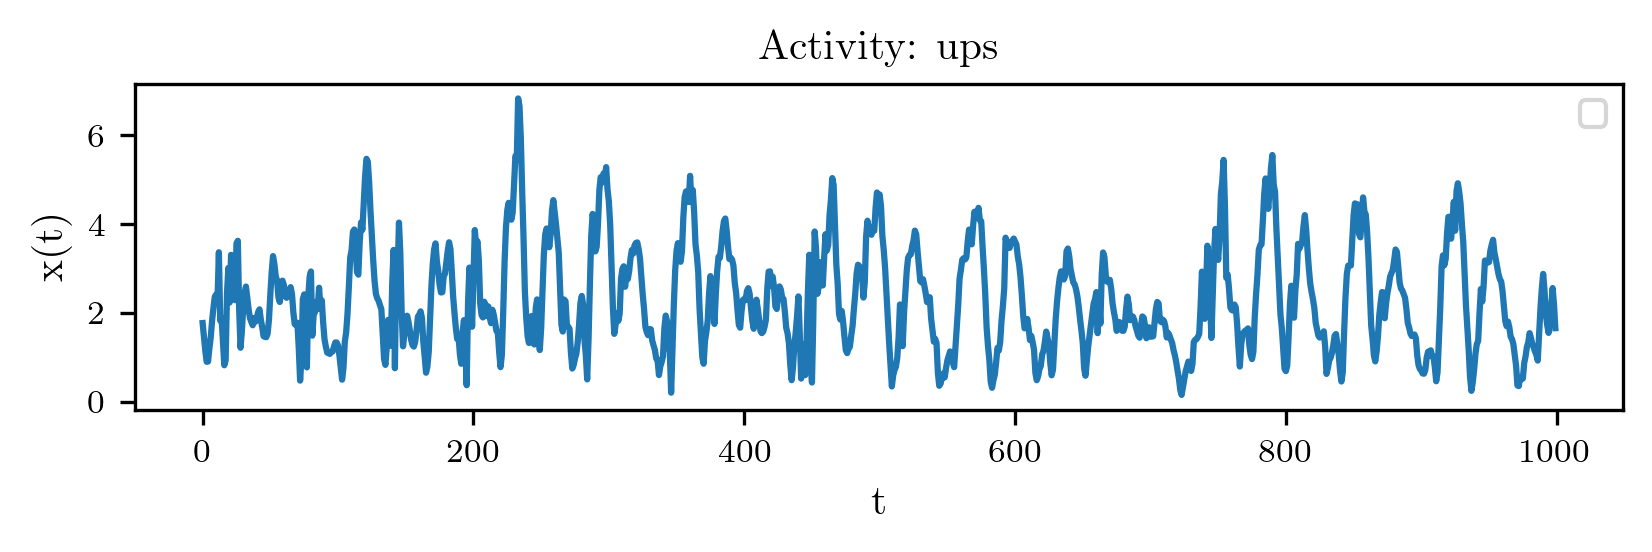
\includegraphics[width=0.49\textwidth, keepaspectratio]{img/dws_example}
			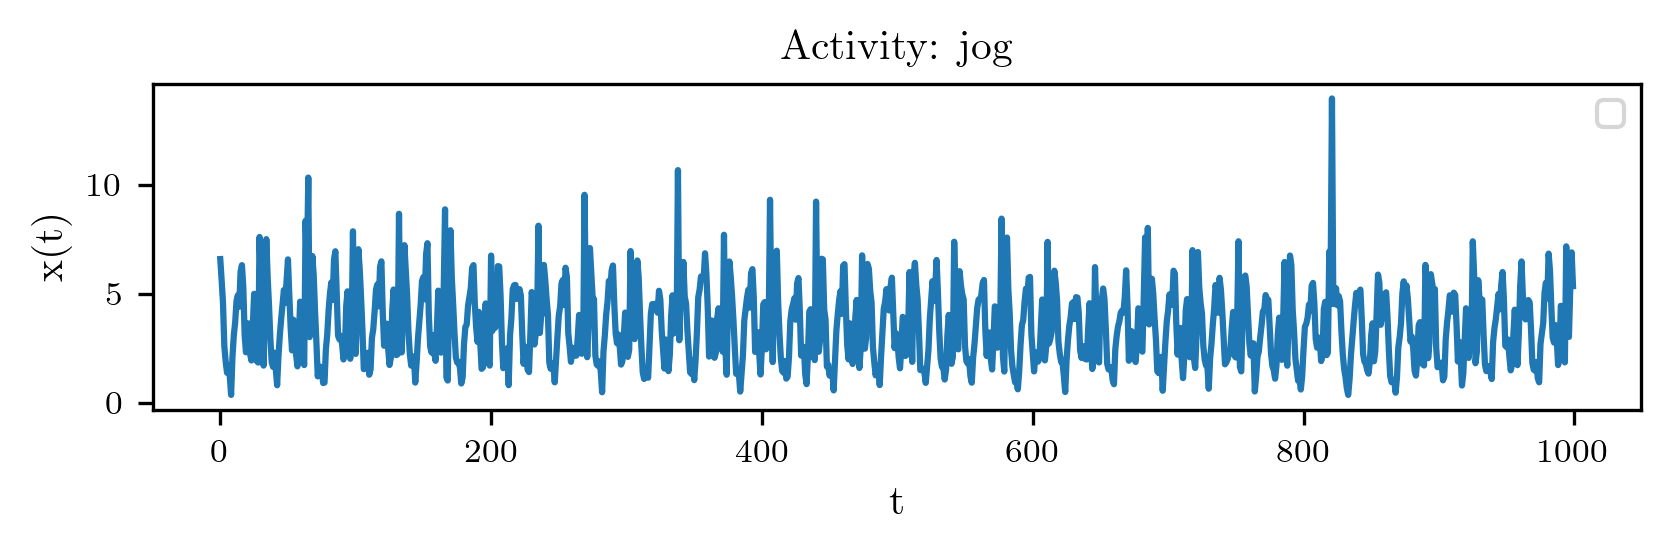
\includegraphics[width=0.49\textwidth, keepaspectratio]{img/jog_example}
			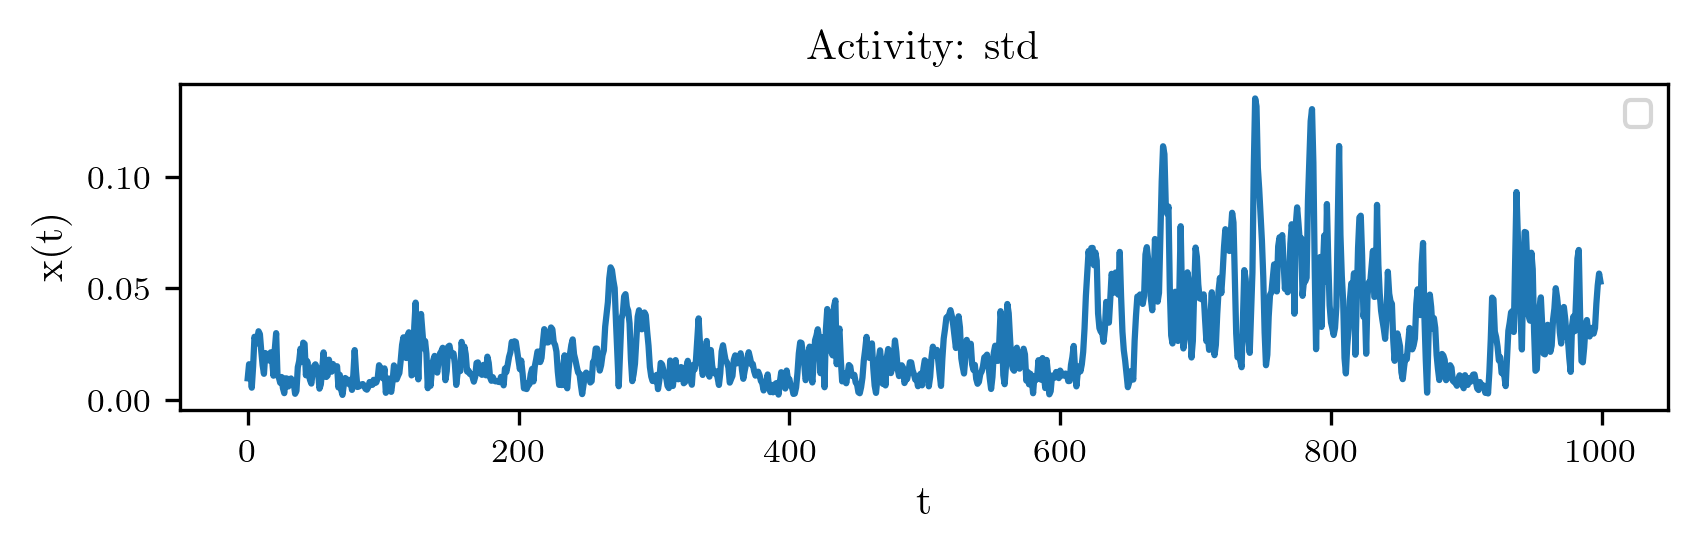
\includegraphics[width=0.49\textwidth, keepaspectratio]{img/stand_example}
			\caption*{Time series from different systems}
		\end{figure}
		
	\end{frame}% say tilde means noised
	
	\begin{frame}{Classification overview}
		
		\begin{enumerate}
			\item Reconstruct (if needed) diffeomorphic phase trajectories from the observed time series: Whitney or Takens embedding theorem.
			\begin{equation*}
				\{\tbx(t_i)\} \to \{\bbx(t_i)\}
			\end{equation*}
			\item Learn (if not provided) vector fields of the systems $f_i(\bz)$ from the trajectories (NODE).
			\begin{equation*}
				\hat{f} = \underset{f \in \mathcal{F}}{\arg\min} \  \mathcal{L}(\{\bx(t_i)\}, f)
			\end{equation*}
			
			Choose $\mathcal{L}, \mathcal{F}$ according to the prior knowledge of the system.			
			\item Associate a test trajectory with the system that gives least deviation from the \emph{initial value problem} (IVP) (\ref{eq:lat_dyn}).
			
			\begin{equation*}
				k = \underset{k \in 1 \ldots K}{\arg\min} \  \rho \big( \{\bx(t_i)\}, \text{IVP}(t_i, f_k, \bbx_0) \big)
			\end{equation*}
		\end{enumerate}
		
	\end{frame}
	
	\begin{frame}{Approach limitations}
		
		In steps 2-3 we need to compute precise IVP trajectories and know exact $\bbx_0$. On practice, it is not possible for several reasons
		
		\begin{enumerate}
			\item In many cases IVP has no analytic solution and \emph{numerical solvers} are used. They induce numerical error and may have stability issues.
			\item Learned field $\hat{f}$ from step 2 is an approximation of the real $f$. It contributes to the IVP error.
			\item Observed series $\bx_{t_i}$ are noisy including starting point $\bbx_0$.
			\item The dynamical system (\ref{eq:lat_dyn}) may not be an adequate time series model globally. For example, the SDE model may be more appropriate
			\begin{equation}\label{eq:series_sde_dyn}
				\begin{cases}
					d\bbx(t) = f(\bbx)dt + G dW(t), \\
					\bbx(0) = \bbx_0,
				\end{cases}
			\end{equation}
		\end{enumerate}
		
	\end{frame}
	
	\begin{frame}{Classification as the filtering problem}
		
		We use ODE solvers to approximate dynamics (\ref{eq:lat_dyn}) and obtain the following state space model
		\begin{gather*}
			\bbx_{t_{i+1}} = \text{ODESolve}(\bbx_{t_i}) \\
			\bx_{t_i} = \bbx_{t_i} + \epsilon_{t_i} \\
			\bbx_0 \sim F(x)
		\end{gather*}
		In this formulation we change $\text{IVP}(t_i, f_k, \bbx_0)$ for $\mathbb{E}[ \{ \bbx_{t_i} \} | \{ \bx_{t_i}, \bbx_0 \}]$ --- the filtering problem. The classifier is now
		\begin{equation*}
			k = \underset{k \in 1 \ldots K}{\arg\min} \  \rho \big( \{\bx(t_i)\}, \mathbb{E}[ \{ \bbx_{t_i} \} | \{ \bx_{t_i}, \bbx_0 \}] \big).
		\end{equation*}
		
		For the SDE dynamics we just obtain more general filtering problem
		\begin{gather*}
			\bbx_{t_{i+1}} = \text{ODESolve}(\bbx_{t_i}) + \xi_{t_{i+1}} \\
			\bx_{t_i} = \bbx_{t_i} + \epsilon_{t_i} \\
			\bbx_0 \sim F(x)
		\end{gather*}
		
	\end{frame}
	
	\begin{frame}{Experiments to justify filtering}
		
		Compare direct ODE solvers and filtering for the noisy trajectory of the ODE system $\dot{x} = x$
		
		%\vspace{-1.5em}		
		\begin{figure}[h]
			\centering
			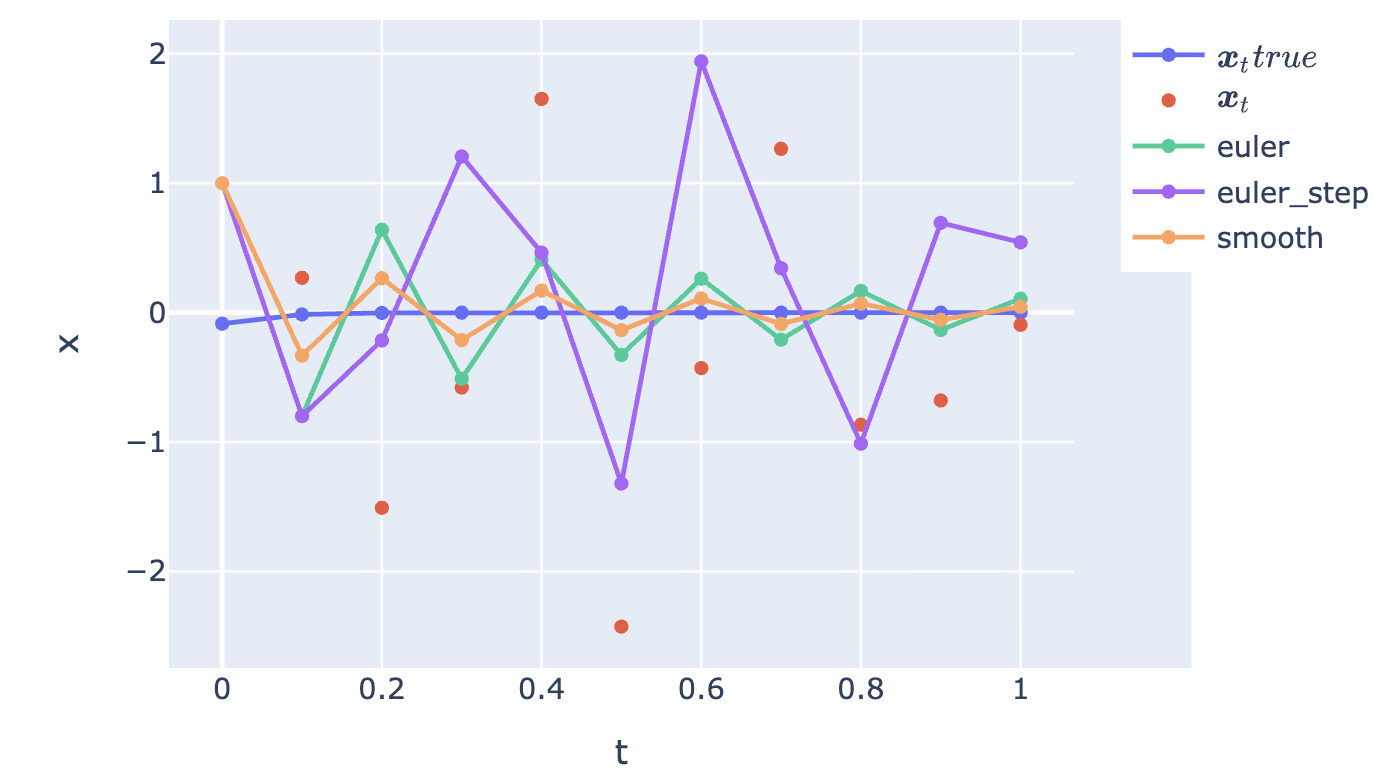
\includegraphics[width=0.49\textwidth, keepaspectratio]{img/Screenshot 2026-05-23 at 15.28.58.png}
		\end{figure}
		
		Compare direct ODE solvers and filtering for the noisy trajectory of the SDE system $dx_t = x_t (1 + dW_t)$
		
		%\vspace{-1.5em}
		\begin{figure}[h]
			\centering
			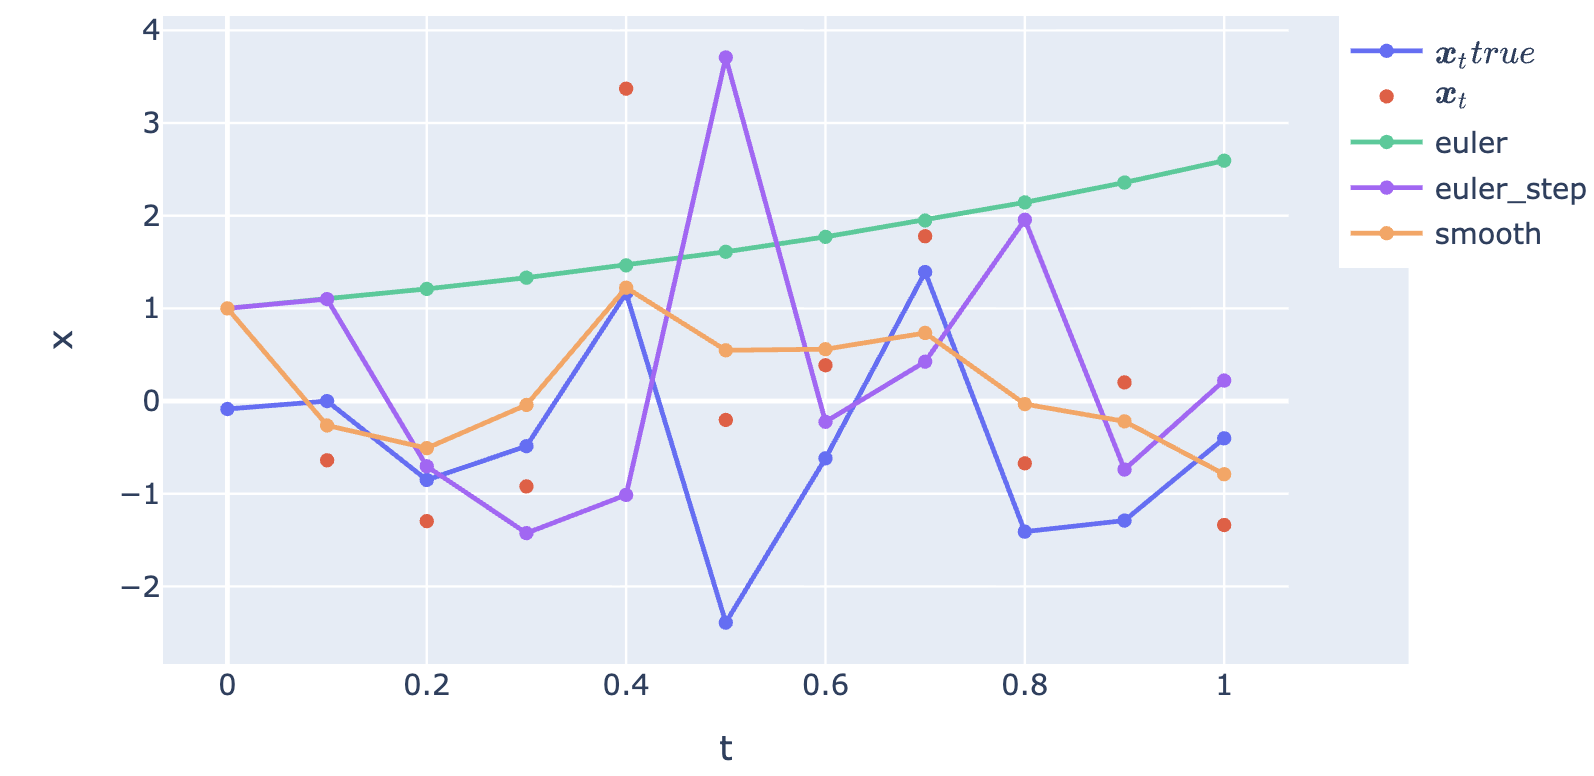
\includegraphics[width=0.49\textwidth, keepaspectratio]{img/Screenshot 2026-05-23 at 15.35.19.png}
		\end{figure}
		
	\end{frame}
	
	%\begin{frame}{Experiment on classifying IMU}
	%	
	%\end{frame}
	
	\begin{frame}{Выносится на защиту}
		
		\begin{enumerate}
			\item Предложен метод классификации временных рядов в модели ODE/SDE с учётом случайного шума.
			\item Получены теоретические результаты асимптотической оптимальности классификатора при достаточной информации о дин.системах и начальной точки. Обоснован подход с фильтрацией при отсутствии данных условий.
			\item Подход эмпирически валидирован на синтетических и реальных данных.
		\end{enumerate}
		
	\end{frame}
	
\end{document}